\chapter{Verification and validation}
\label{ch:results}
% Validation: Are we building the right system?
% Verification: Are we building the system right?

To verify if running all Tribler functionality on mobile devices is feasible we take a look at relevant performance characteristics.
We take several measurements to quantify how well it works in terms of our non-functional requirements.
%TODO Measure waar staan we nu, wat is er mogelijk
%Functionality: Meet requirements in implementation
%Device vs PC
%Device vs device

For scale a laptop and PC are included in some measurements.
We focus on the design aspects and evaluate the key performance indicators:
\begin{itemize}
	\item{\emph{scalability} in terms of discovery time and bandwidth accounting.}
	\item{\emph{performance} in terms of frequency and duration of function calls, in terms of latency and startup time,}
	\item{\emph{resource usage} in terms of CPU utilization,}
\end{itemize}

% Rationale
% Metrics
% Expected / desired results
% Setup
% Results
% Conclusions


\section{Content discovery}
%TODO: 2 subvragen: creation "req.X" (8) & adding "req.Y" (8) & discovery "req.Z" (15)
% laat zien dat linair verband aannemelijk is voor creation & adding
%TODO: acquisitie van data uitbreiden
%meta info does not scale with content size
%TODO: remove times from schematic scenario figure
% Rationale
New content is generated on the device, like for example a video that has been recorded.
Before anyone can view that content it has to be added to a channel and discovered by other devices.
% Metrics
We measure the amount of time it takes for other devices, which are subscribed to the channel, to discover new content.
We also measure the amount of time it takes for content to be added to a channel in the form of a torrent.
The amount of time it takes for a torrent to be created is relative to the size of the content.
Therefore these measurements are normalized to a file of 1 MB.
% Expected / desired results
Depending on the random walk in the channel's community content can be discovered either very quickly or after a while due to property of eventual consistency.
% Setup
On one Nexus 6 device a channel is created to which 13 other devices subscribe via NFC.
Then repeatedly a new video is recorded and added to that channel.
A content discovered event is registered on each device individually and all devices are synced with NTP.
Each device is connected to the same WLAN and within 1 to 2 meters distance from the access point.
\begin{figure}[H]
	\centering
	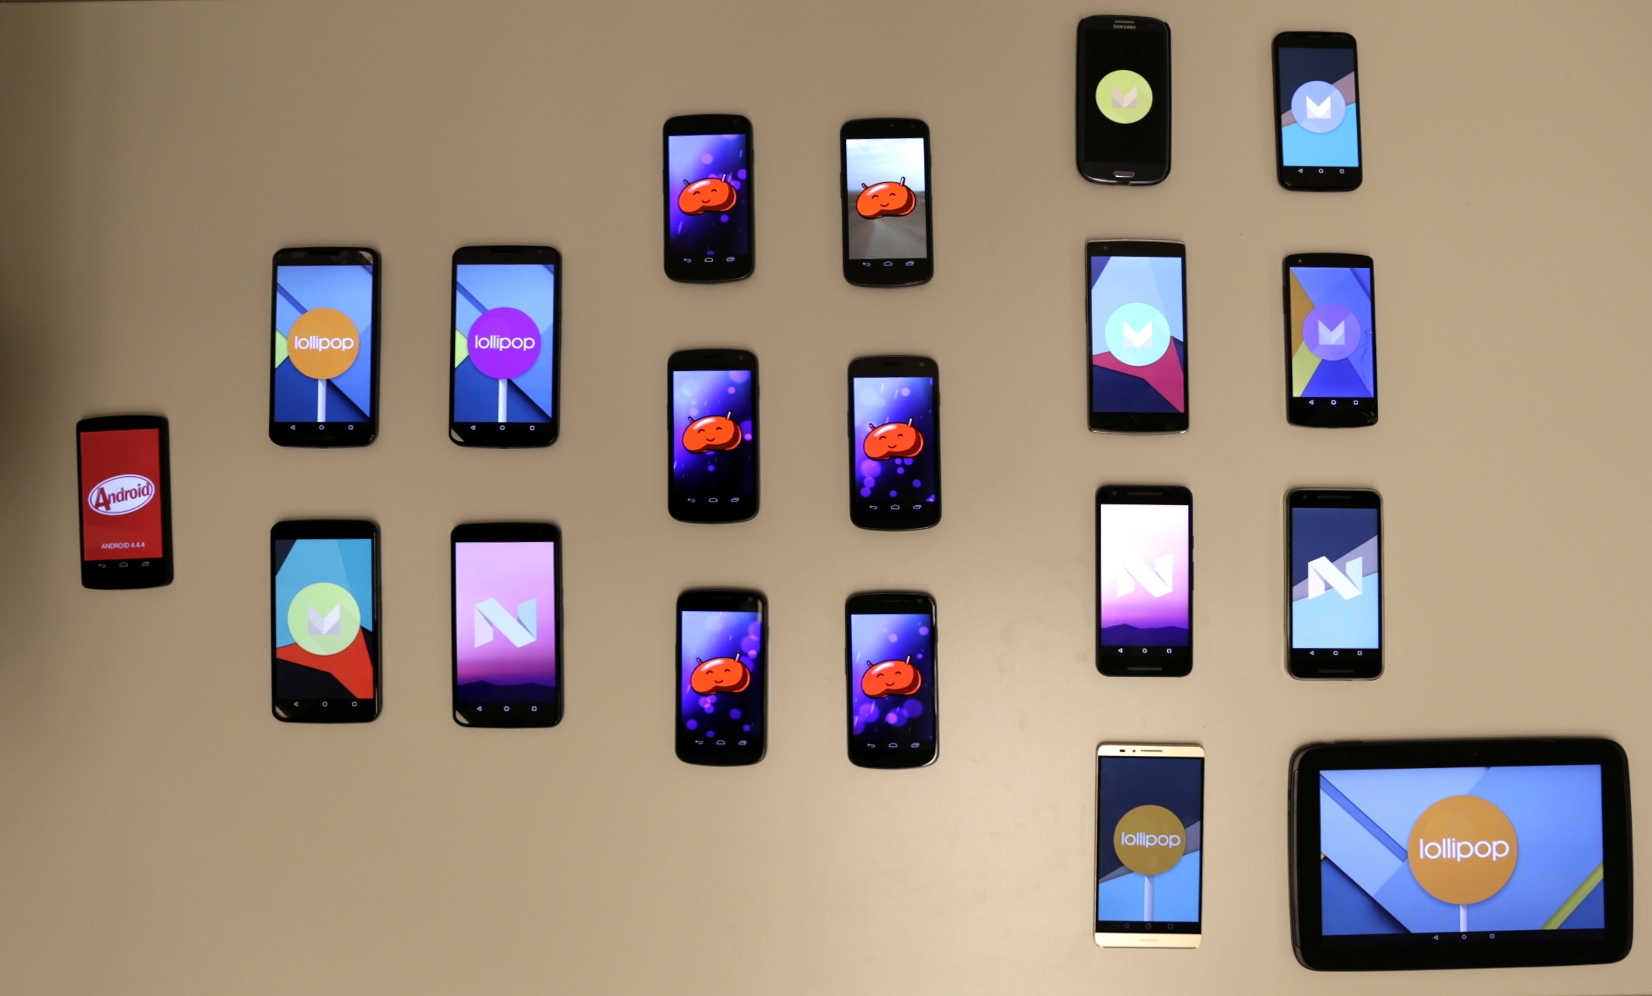
\includegraphics[width=\textwidth]{phones_2}
	\caption{All devices used in the experiment showing the about Android screen.}
	\label{fig:phones_2}
\end{figure}
% Results
\begin{figure}[H]
	\centering
	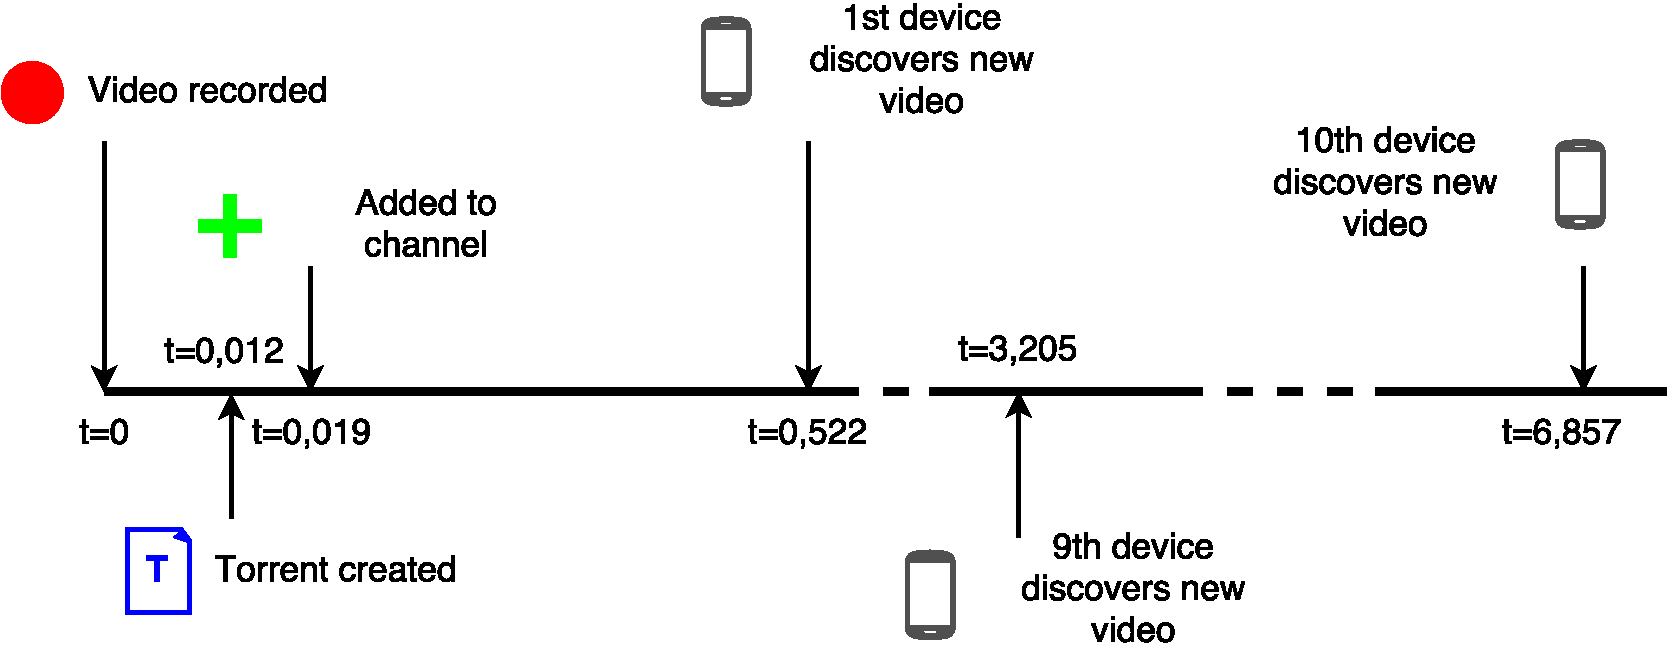
\includegraphics[width=\textwidth]{content_dissemination}
	\caption{Sequence of events with time values from median of results.}
	\label{fig:content_dissemination}
\end{figure}
Figure \ref{fig:boxplot-nr.of.devices-130} shows the amount of time it takes a number of devices to discover new content on a subscribed channel.
\begin{figure}[H]
	\centering % trim={<left> <lower> <right> <upper>}
	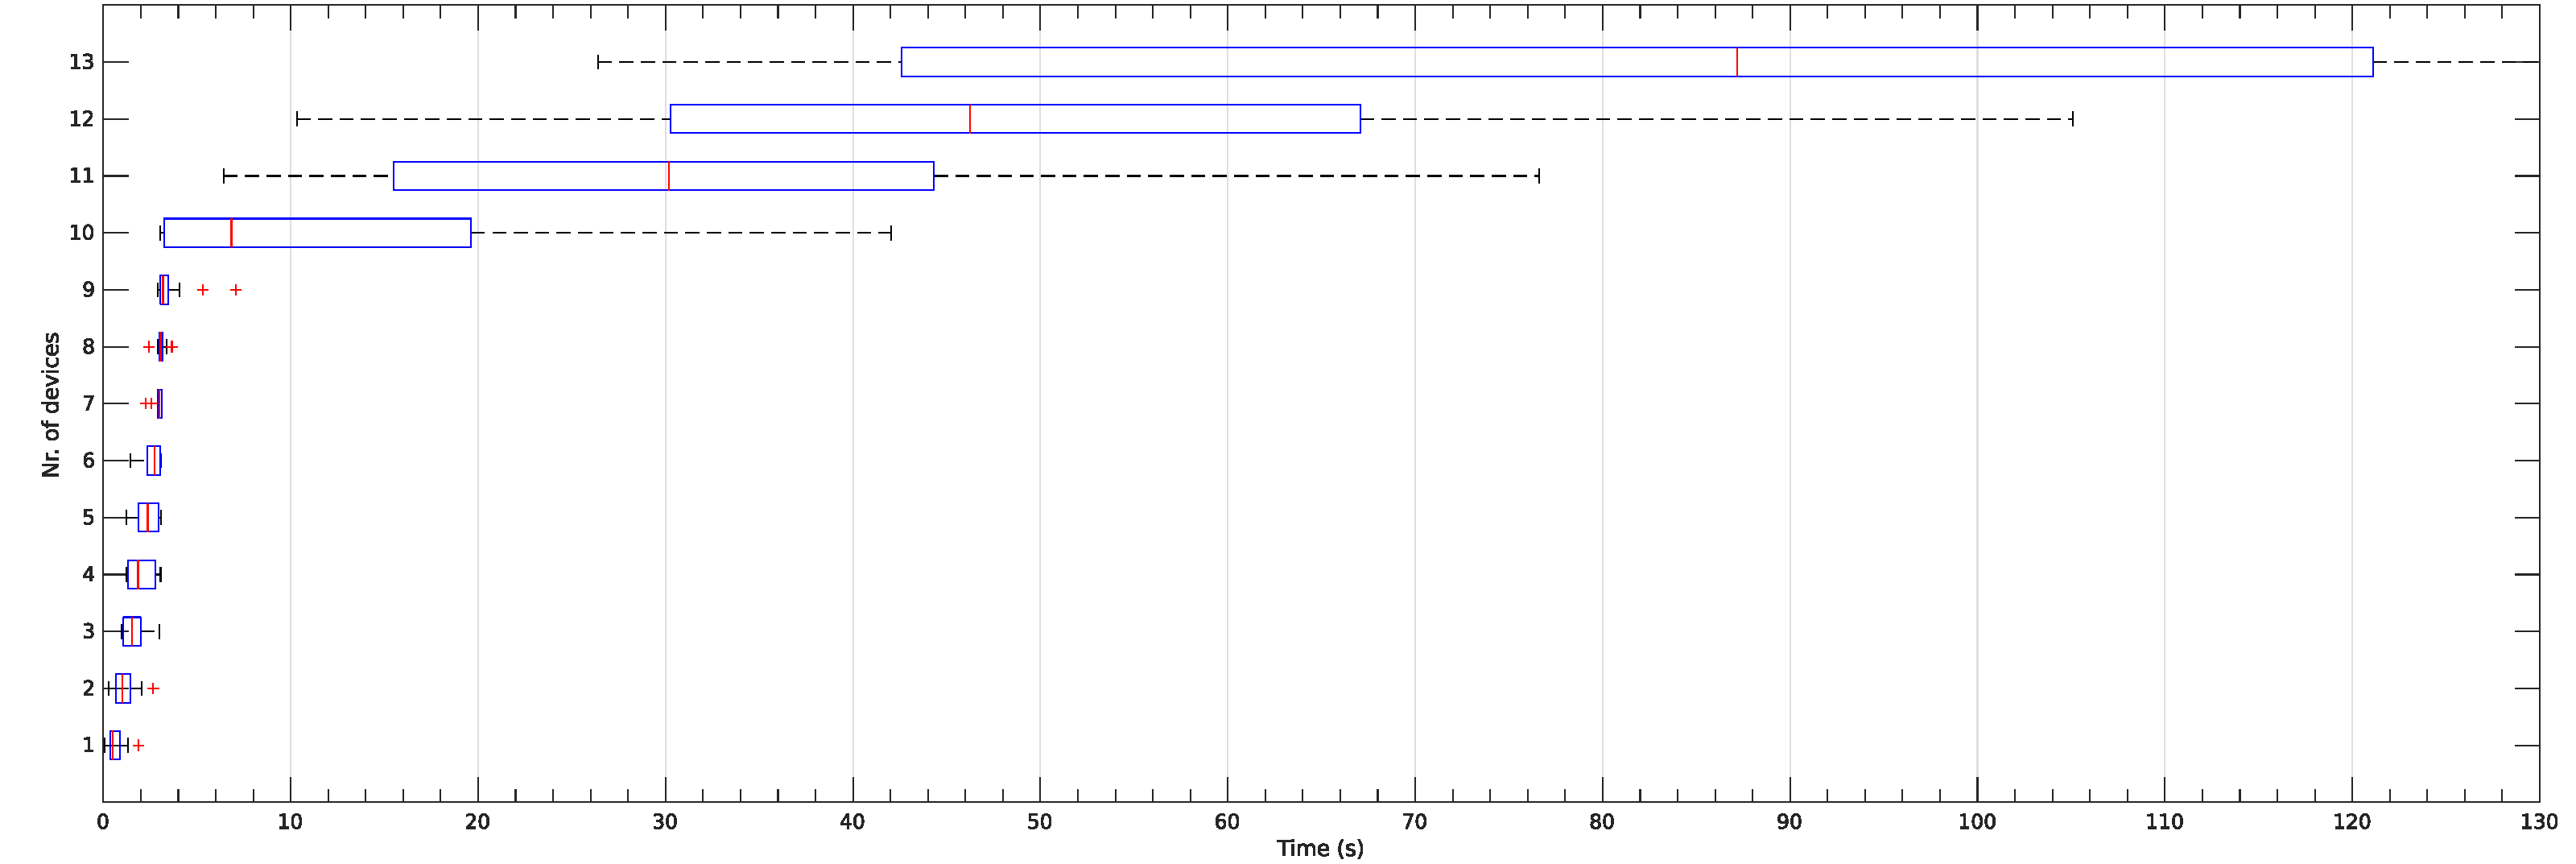
\includegraphics[trim={0.9cm 0 0 0},clip,width=\textwidth]{boxplot-nrofdevices-130}
	\caption{Elapsed time from adding new content to a channel and it being discovered by subscribed peers.}
	\label{fig:boxplot-nr.of.devices-130}
\end{figure}
\begin{figure}[H]
	\centering
	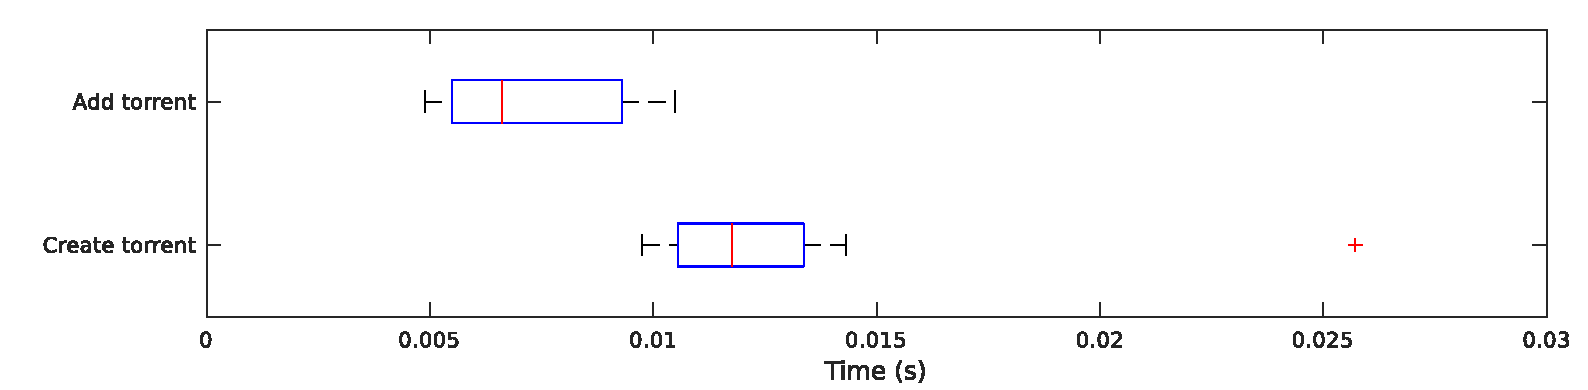
\includegraphics[width=\textwidth]{boxplot-per-mb-torrent-create-add}
	\caption{Time required to create a torrent and add it to a channel, normalized for 1 MB of content.}
	\label{fig:boxplot-per-mb-torrent-create-add}
\end{figure}
The results show that within 4 seconds 9 devices have discovered the new content.
From the 10th device and beyond an increase in discovery time is noticeable.
% Conclusions
This could be explained by the fact that only 10 peers are connected at the a time.
Much more peers are needed to give an accurate representation in terms of scalability.
What can be concluded from this experiment is that on the same local network the first device discovers the new content in less than 2 seconds.
From the 10th device onwards the dissemination slows down.


\section{Multichain performance}
% Rationale
Multichain is the new accounting system of Tribler.
This feature is central to the concept of trust in the Tribler network and is very important for the future as other functionality will be built upon it.
If mobile devices are to become full-fletched nodes on the network they must support this feature.
With Multichain any peer registers the bandwidth it exchanges with other peers.
It aggregates these exchanges in blocks and signs them like a receipt and sends that to the other party to sign as well.
These blocks are linked in a block-chain to foil attempts of cheating the system.

Multichain is explicitly designed to not use a global state.
Syncing a global state is less scalable in terms of storage and network bandwidth.

% Metrics
The creation and signing of these blocks is measured to determine if it scales well.
Multichain signs a block every 10 minutes, meaning our experiment of generating 25.000 blocks represent about half a year (173,6 days) of continuous effort.
% Expected / desired results
The database containing these blocks will grow over time, but should not slow down too much because of it.
% Setup
Measurements were taken on six different devices on multiple moments during development.
% Results
Figure \ref{fig:multichain_25} show the performance graphs of every measurement.
\begin{figure}[H]
	\centering
	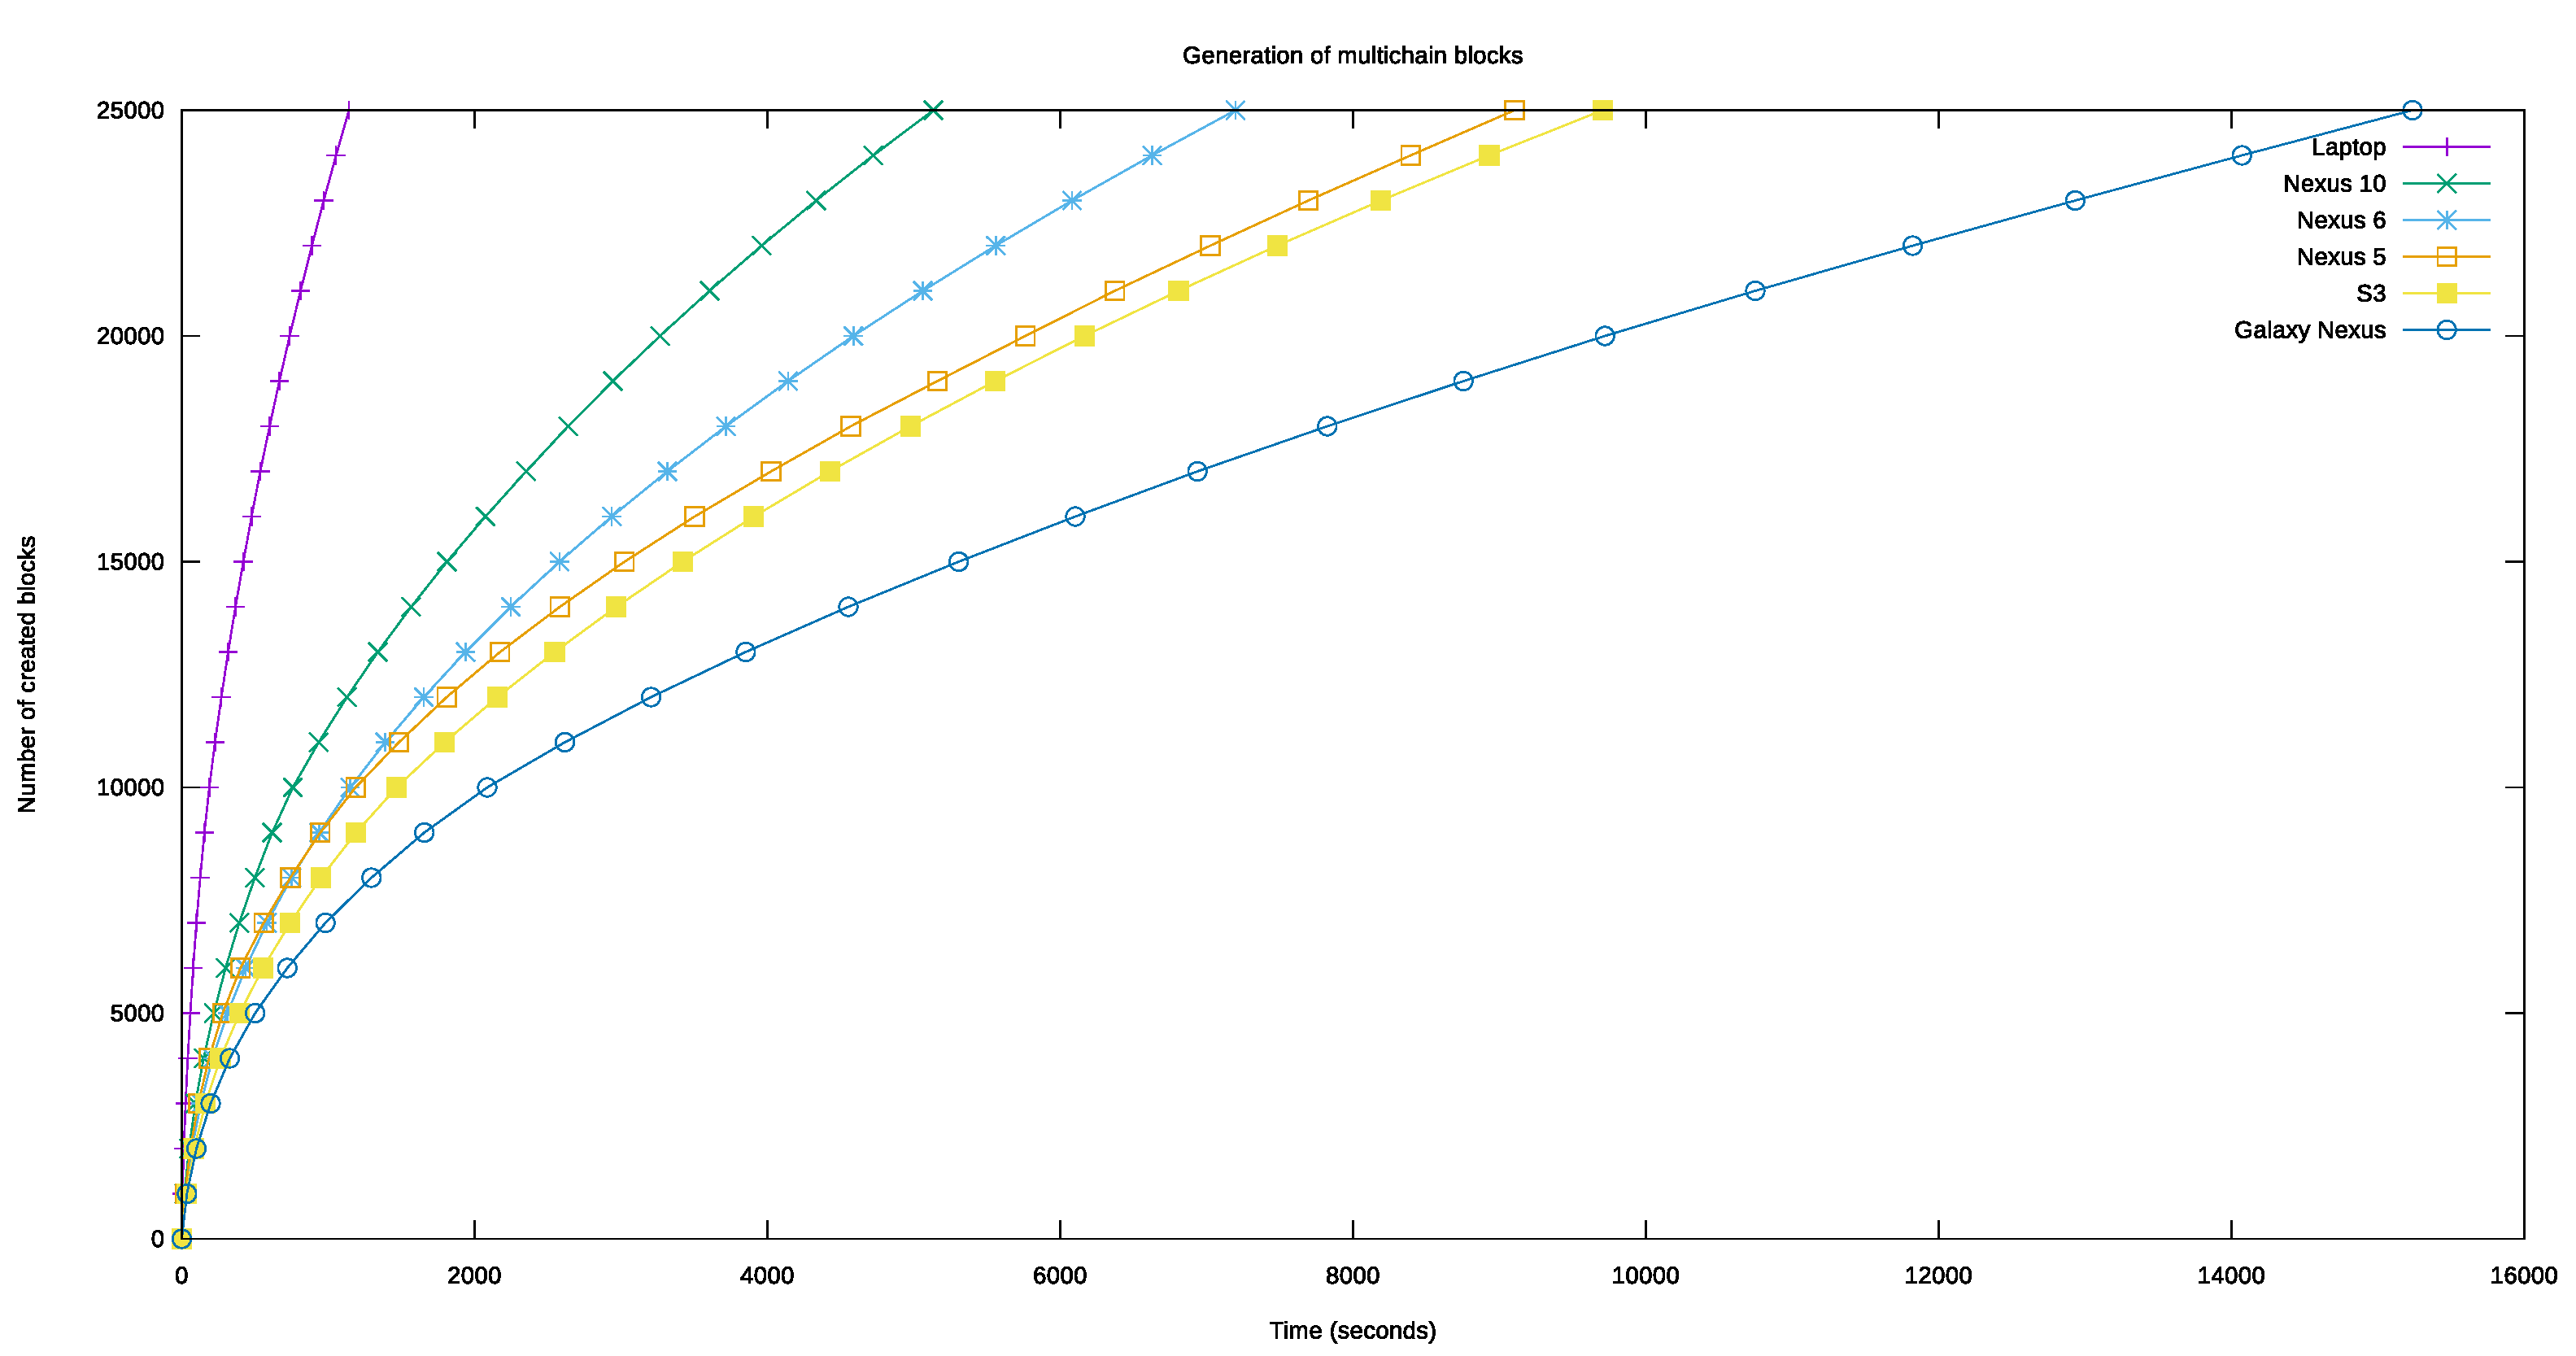
\includegraphics[width=\textwidth]{multichain_scale_2599_25k}
	\caption{Creating and signing of 25.000 blocks between two peers}
	\label{fig:multichain_25}
\end{figure}
Clearly visible from the graphs is that Multichain does not scale linearly on any device.
They also show that mobile devices are at least a factor of two slower than an ordinary laptop and scale worse.
% Conclusions
Due to the nature of block-chain every new block needs to contain the hash value of the previous block.
If a database lookup is needed for this and the database is growing, that can explain the non-linear course of the graph.
This can be easily resolved by keeping the last hash value for currently connected peers in memory.
However this is an indication that creating blocks by the thousands is an IO bound process, rather than CPU bound.
Finally, if mobile devices are to be full-fletched nodes on the Tribler network, they should not slow down significantly more than any other ordinary laptop, besides being slower in the first place.
Hardware acceleration could close this gap without sacrificing battery life too much.
Because mobile devices are a bit behind on the technology curve with respect to desktop computers it is probable that the gap becomes smaller over the coming years.
The capacity to store enough Multichain blocks to audit past exchanges should also be on par.
If not, other more powerful nodes could be queried to supply the necessary history about a peer, that requests your bandwidth, to verify if that peer is trustworthy.


\section{Startup time}
%TODO previous chapter: implementation architecture startup sequence nice design, how does it perform?
% when is gui ready for real? do not say gui is response blabla because we do not measure.

% Rationale
Key to user retention is a fast startup time.
Therefore the service starts up in the background, separately from the GUI.
This way at the GUI is responsive to user input while the service may still be loading.
One of the design objectives for separating the front-end from the back-end was responsiveness.
However before any task can be executed by the service it needs to be actually started.
% Metrics
To measure the startup time we register the time of launching the app and the moment the Tribler-started-event occurs.
This event is sent over the API event-stream and signifies that Tribler is fully started and ready to accept all incoming requests.
% Expected / desired results
We expect consistent loading times because right after starting we shut Tribler down again.
% Setup
%TODO consistency within device
%consistency over different devices, explain
To get a good idea of how the user experience may differ we measure the startup time 10 times on 5 different devices.
The app is launched with Android Debug Bridge (adb) from a laptop and the Tribler-started-event is read from logcat over adb and timed on the same laptop so they use the same clock.
% Results
\begin{figure}[H]
	\centering % trim={<left> <lower> <right> <upper>}
	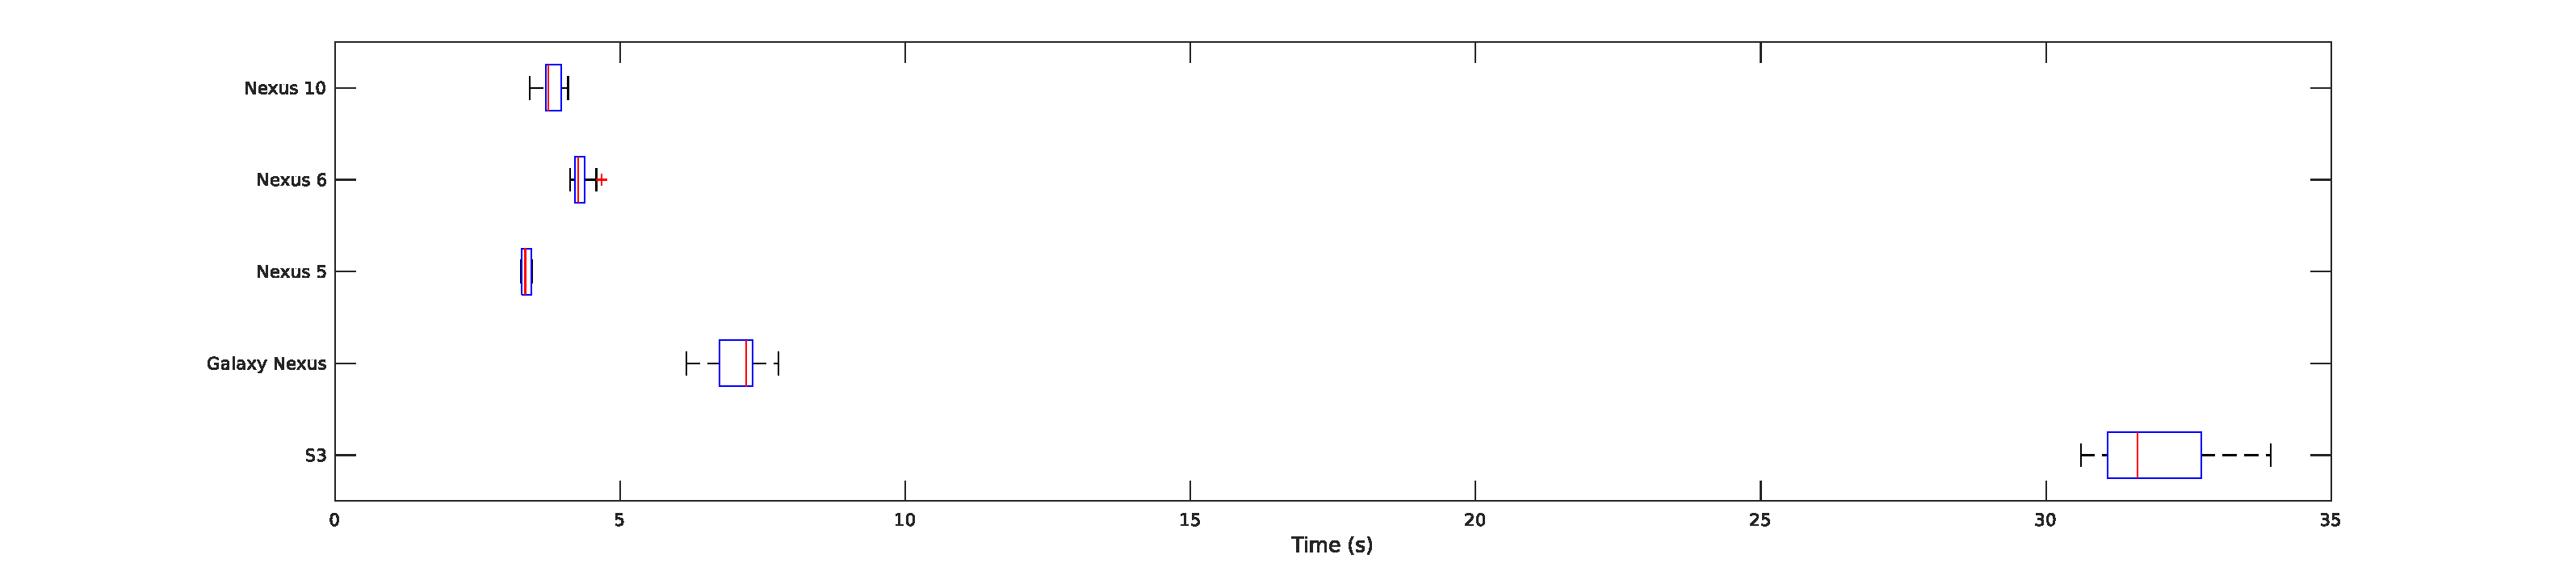
\includegraphics[trim={4cm 0cm 4cm 0cm},clip,width=\textwidth]{boxplot-startup}
	\caption{Startup times per device}
	\label{fig:boxplot-startup}
\end{figure}
Table \ref{table:startup_time} shows the statistics per device.
\begin{table}
	\begin{tabular}{l | *{5}{r}} \hline
		Device & N & Avg. (s) & Min. (s) & Max. (s) & s (s) \\ \hline \hline
		Nexus 10        & 10 & 3.781 & 3.416 & 4.085 & 0.211 \\ \hline
		Nexus 6          & 10 & 4.319 & 4.124 & 4.670 & 0.179 \\ \hline
		Nexus 5          & 10 & 3.353 & 3.273 & 3.459 & 0.081 \\ \hline
		Galaxy Nexus & 10 & 7.086 & 6.161 & 7.772 & 0.454 \\ \hline
		S3                   & 10 & 31.935 & 30.616 & 33.940 & 1.116 \\ \hline
	\end{tabular}
	\caption{???}
	\label{table:startup_time}
\end{table}
The results show a very small sample standard deviation and a very low startup time.
The S3 is performing worse than may be expected judging from the results of the other devices.
% Conclusions
The reason for that may be that this phone was not wiped and given a fresh install of Android.
That could mean that other applications installed on a device could significantly impact the performance of Tribler.
The sample standard deviation is relatively small though, which contradicts this hypothesis.
This should be investigated further, including if anything can be done on the part of Tribler.


\section{Content creation}
%TODO
%grote scenario


\section{API latency}
% Rationale
The user expects operations to take a consistent and reasonable amount of time.
By design all functionality is going through the API.
% Metrics
We use Apache JMeter to verify if the API is responding consistently within a reasonable amount of time by measuring the latency.
JMeter measures the latency from just before sending the request to just after the first response has been received. \cite{jmeter_glossary}
Thus the measurement includes the time needed to assemble the request as well as processing it and returning a response with latency on the way back.
It excludes the transfer time of the complete response and subsequent processing and rendering time.
Any client can process and render a response differently, possibly in a streaming fashion.
By leaving out that element this metric is measuring the operation time via the API.
% Expected / desired results
We want to see that the latency is bounded, consistent and generally low.
Previous research has shown the following results on a computer:
\begin{figure}[H]
	\centering % trim={<left> <lower> <right> <upper>}
	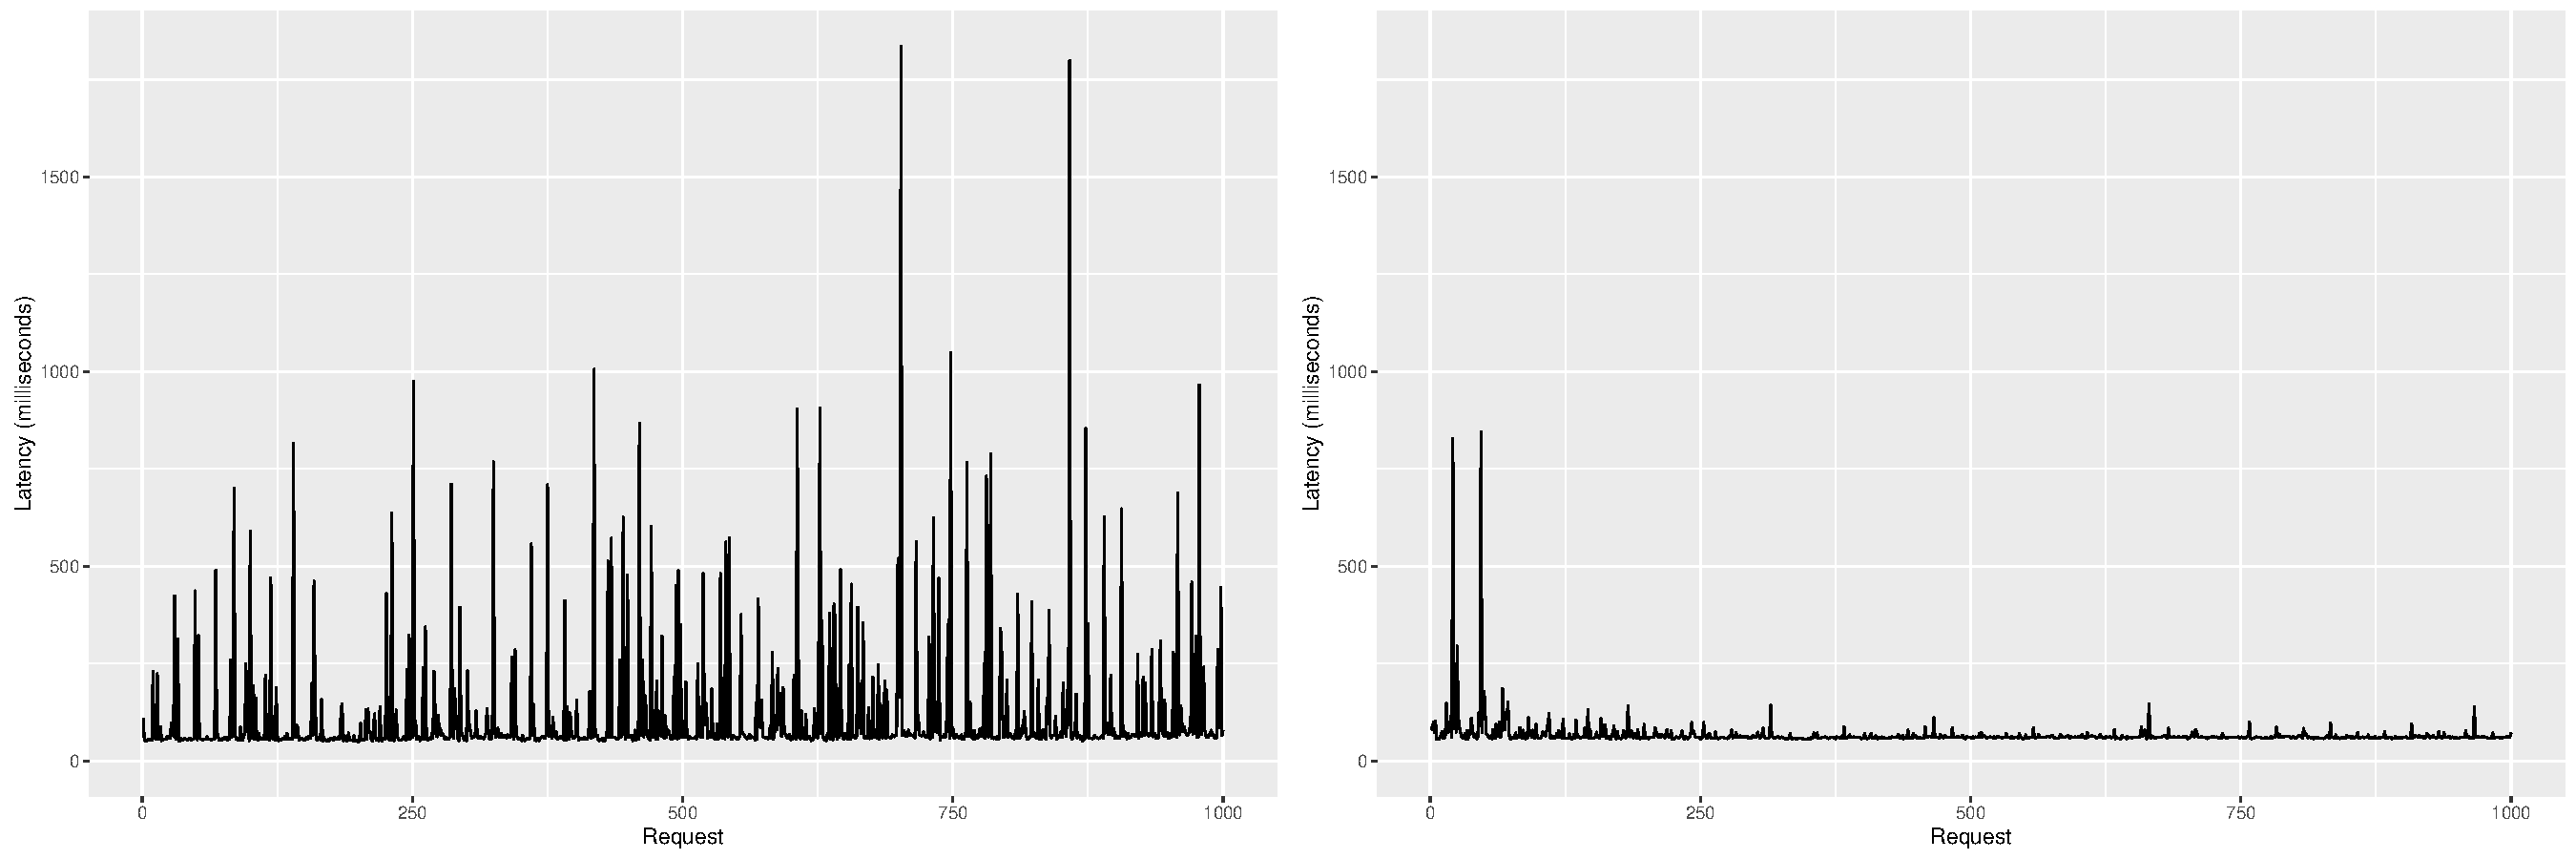
\includegraphics[trim={0 0 23cm 0},clip,width=0.9\textwidth]{api_laurens}
	\caption{API latency on PC}
	\label{fig:api_laurens}
\end{figure}
% Setup
We did the same benchmark with a slightly different setup.
A Nexus 6 smart-phone with Android 6.0.1 Cyanogen mod was connected via USB to a laptop running JMeter.
The API tcp-port was forwarded with ADB.
With JMeter we request the discovered channels from the API a 1000 times and measure the latency.
JMeter is also capable of setting a desired number of requests per minute, provided the device can handle it.
We set this parameter to 300 requests per minute, equal to the other benchmark.
% Results
Our database to be queried is not equal to one used in figure \ref{fig:api_laurens}.
The following figure shows the latency for every request.
\begin{figure}[H]
	\centering
	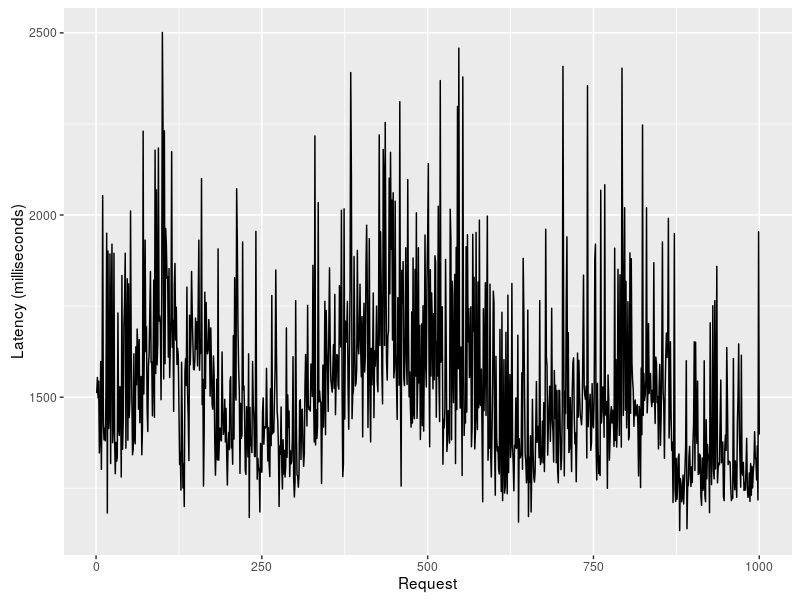
\includegraphics[width=0.9\textwidth]{api_benchmark}
	\caption{API latency on Nexus 6 smart-phone}
	\label{fig:api_benchmark}
\end{figure}
The plot shows large spikes and seemingly a curious and unexpected pattern.
Table \ref{table:api_benchmark} shows the large difference in statistics.
PC is added for reference.
\begin{table}
  \begin{tabular}{l | *{8}{r}} \hline
  	 & N & Avg. (ms) & Min. (ms) & Max. (ms) & $\sigma$ (ms) & Throughput & KB/second & Avg. Bytes \\ \hline \hline
	Nexus 6 & 1000 & 1803 & 1292 & 3292 & 301.25 & 33.3 req/minute & 347.44 & 641709.0 \\ \hline
	PC         & 1000 & 5        & 3      & 107    & 4.42     & 140.8 req/second & 2548.00 & 18525.0 \\ \hline
	Laptop  & 1000 & 101    & 3       & 1712  & 137.70 & 1.0 req/second     & 117.27 & 120042.2 \\ \hline
	Nexus 6 & 1000 & 3975 & 8       & 39477 & 5362.51 & 14.4 req/minute & 49.19 & 210506.8 \\ \hline
	Laptop   & 1000 & 65     & 1       & 1021    & 99.00 & 1.0 req/second      & 73.72 & 75410.6 \\ \hline
	Nexus 6 & 1000 & 1671 & 1390 & 2925 & 174.14 & 35.9 req/minute & 345.94 & 592649.8 \\ \hline
	Laptop   & 1000 & 181   & 101   & 416   & 42.72   & 1.0 req/second   & 579.49 & 592791.3 \\ \hline
  \end{tabular}
  \caption{These numbers are based on elapsed time, not latency, from the entire benchmark}
  \label{table:api_benchmark}
\end{table}
The set rate of 300 requests per minute is clearly not reached by the smart-phone in our benchmark by a factor of 9.
The difference in amount of response data turned out to be much bigger than expected with a factor of 35.
% Conclusions
%TODO: IO bound + crappy Python code WHY?
% busy Twisted reactor?
Tribler uses the event-driven networking engine Twisted, which is also written in Python.
Twisted allows you to build inter-process communication protocols and provides a HTTP server which was used to build the REST API.
Twisted uses a single thread to coordinate all others, called the reactor thread.
If this thread is busy, the REST API can not receive incoming requests resulting in timeouts.

Considering the difference in amount of response data and the bandwidth of USB versus internal memory it is an unfair comparison.
However, based on our result we may conclude that the API does not respond consistently and appear to behave differently than the other benchmark.
The device not being able to process 5 requests per second possibly reveals information about the connection bandwidth and the multi-threaded processing capability.
We assume that the 480MB/s theoretical bandwidth of USB2.0 is not a bottleneck considering the 2,5 MB/s result of the PC.
Being a mobile device also other aspects my be at play here, like CPU frequency scaling.
However this was turned off by acquiring a wake lock from the Android OS.
It appears then that our design approach still suffers from performance issues due to imperfect multi-threaded performance.
Because if the CPU is simply not powerful enough we expect to see a linear pattern instead of what we actually see in \ref{fig:api_benchmark}.
This phenomenon is not of great importance though, because users are not expected to fire hundreds of requests per minute to the API.
Further investigation should figure out if this phenomenon is also observed with lower amounts of requests per minute.


\section{Profiling}
% Rationale
Because of the challenges put forward in chapter \ref{ch:tribler_mobile} we investigate if time is spent disproportionately on some function.
% Expected / desired results
We expect that the limited resources of a mobile device may impact particular features more than others.
If hardware acceleration is not present the less powerful CPU may struggle with encryption tasks.
% Metrics
Instead of CPU time, time actually spent processing by the CPU, we measure wall-clock time.
This way we measure the amount of time a user would have to wait for a certain function to be executed.
%TODO
We focus on wall clock time instead of CPU time because...

% Setup
With the cProfile Python module and the visualisation tool SnakeViz we can see if any function takes a disproportionate amount of time.
A Nexus 6 smart-phone with Android 6.0.1 Cyanogen mod was used for profiling Tribler.
The profiler was running for 10 minutes with Tribler during normal operation and without any user input.
% Results
\begin{figure}[H]
	\centering
	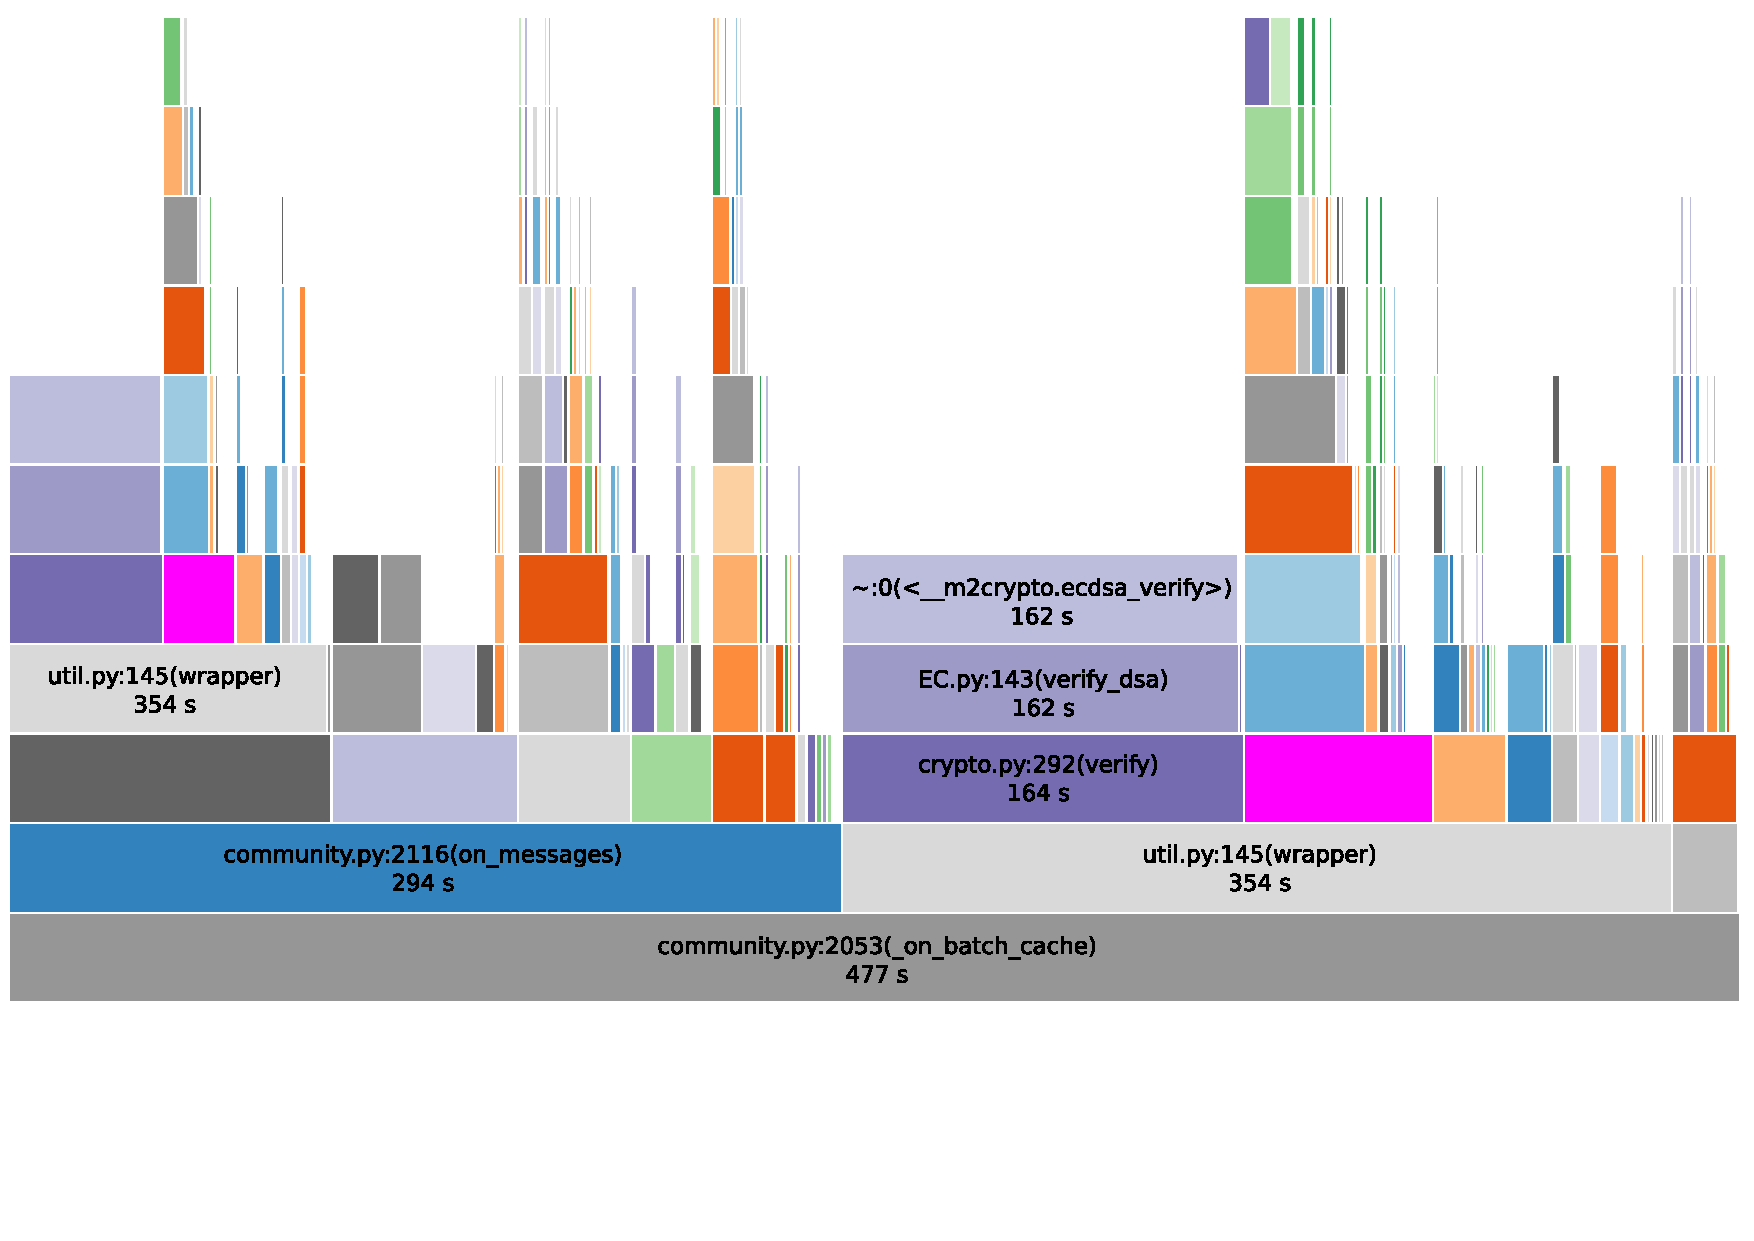
\includegraphics[width=\textwidth]{profile_1468515157-2}
	\caption{Profiler results of 10 minutes Tribler run time (bright pink represents business logic upon receiving a torrent)}
	\label{fig:profile}
\end{figure}
\begin{table}
	\begin{tabular}{*{3}{r} | l} \hline
		\# Calls & Total time (s) & Time per call (s) & Function \\ \hline \hline
		15 & 0.4867 & 0.03245 & method 'commit' of 'sqlite3.Connection' objects \\ \hline
		1 & 0.01692 & 0.01692 & method 'executescript' of 'sqlite3.Cursor' objects \\ \hline
		3820 & 64.28 & 0.01683 & method 'poll' of 'select.epoll' objects \\ \hline
		2 & 0.01048 & 0.005241 & \_\_m2crypto.ec\_key\_gen\_key \\ \hline
		31075 & 162 & 0.005212 & \_\_m2crypto.ecdsa\_verify \\ \hline
		1650 & 7.133 & 0.004323 & \_\_m2crypto.ecdsa\_sign \\ \hline
		1 & 0.001708 & 0.001708 & \_socket.gethostbyaddr \\ \hline
		1 & 0.001284 & 0.001284 & built-in method SSL\_library\_init \\ \hline
		567 & 0.565 & 0.0009965 & method 'executemany' of 'sqlite3.Cursor' objects \\ \hline
		8 & 0.005731 & 0.0009552 & \_\_import\_\_ \\ \hline
		12 & 0.01083 & 0.0009029 & method 'connect\_ex' of '\_socket.socket' objects \\ \hline
		1 & 0.00055 & 0.00055 & built-in method SSL\_load\_error\_strings \\ \hline
		5 & 0.002515 & 0.000503 & method 'recv' of '\_socket.socket' objects \\ \hline
		6989 & 3.436 & 0.0004917 & method 'executemany' of 'apsw.Cursor' objects \\ \hline
		1 & 0.000485 & 0.000485 & dir \\ \hline
		63677 & 20 & 0.000314 & method 'execute' of 'apsw.Cursor' objects \\ \hline
		5546 & 1.38 & 0.0002488 & \_\_m2crypto.ec\_key\_read\_pubkey \\ \hline
		15943 & 3.414 & 0.0002141 & method 'sendto' of '\_socket.socket' objects \\ \hline
		44 & 0.009405 & 0.0002137 & open \\ \hline
		1 & 0.000212 & 0.000212 & built-in method OpenSSL\_add\_all\_algorithms \\ \hline
		2 & 0.000405 & 0.0002025 & \_\_m2crypto.ec\_key\_new\_by\_curve\_name \\ \hline
		2 & 0.000394 & 0.000197 & netifaces.interfaces \\ \hline
		296 & 0.05179 & 0.000175 & method 'sort' of 'list' objects \\ \hline
		5 & 0.000826 & 0.0001652 & \_\_m2crypto.ec\_key\_read\_bio \\ \hline
		1 & 0.000147 & 0.000147 & \_\_m2crypto.rand\_seed \\ \hline
		4 & 0.00058 & 0.000145 & netifaces.ifaddresses \\ \hline
		47 & 0.005664 & 0.0001205 & androidembed.log \\ \hline
		12 & 0.001445 & 0.0001204 & thread.start\_new\_thread \\ \hline
		8 & 0.000936 & 0.000117 & posix.mkdir \\ \hline
		2240 & 0.2615 & 0.0001167 & posix.open \\ \hline
		17 & 0.001964 & 0.0001155 & compile \\ \hline
		3 & 0.00034 & 0.0001133 & \_\_m2crypto.ec\_key\_write\_bio\_no\_cipher \\ \hline
		5553 & 0.6196 & 0.0001116 & \_\_m2crypto.ec\_key\_write\_pubkey \\ \hline
		7 & 0.000777 & 0.000111 & method 'send' of '\_socket.socket' objects \\ \hline
		140069 & 15.4 & 0.00011 & method 'execute' of 'sqlite3.Cursor' objects \\ \hline
		16 & 0.001759 & 0.0001099 & method 'shutdown' of '\_socket.socket' objects \\ \hline
	\end{tabular}
	\caption{Native function calls wall clock time broken down per call during the 10 minute profiling (600 seconds total time)}
	\label{table:profiling_details}
\end{table}
Figure \ref{fig:profile} shows that 27\% of the time is spent on verifying cryptographic signatures.
The bright pink represents the update function, which signifies various business logic upon receiving a torrent.
Also notable is the same stack of functions within and outside of a community on top of the wrapper.
This can be explained by the fact that torrents can be discovered outside of a community too.
%TODO
execute of apsw.Cursor
execute of sqlite3.Cursor
select.epoll \cite{http://stackoverflow.com/questions/2032598/caveats-of-select-poll-vs-epoll-reactors-in-twisted}
% Conclusions
%TODO
The time per call is most important for optimization because...

The significant chunk of time that the crypto takes is as expected.
Since this task is actually delegated to the C library M2Crypto it should be possible to release the GIL of the Python interpreter so other Python code that does not depend on it can be executed.
The main alternative provided in the standard library for CPU bound applications is the multiprocessing module, which works well for workloads that consist of relatively small numbers of long running computational tasks, but results in excessive message passing overhead if the duration of individual operations is short \cite{http://python-notes.curiousefficiency.org/en/latest/python3/multicore_python.html}.
As seen from the time per call for \_\_m2crypto.ecdsa\_verify in table \ref{table:profiling_details} the multiprocessing module would likely cause too much overhead.
%TODO
Another way to optimize is multiprocessing, which avoids the GIL completely \cite{quinten}.

\section{CPU utilization}
%IO bound or CPU bound?
%TODO: tijdens HD streaming: net cpu over, nu nog steeds??
% let it run and measure
We saw in X that the cryptography takes a lot of time.
We need to know if this is CPU bound or not for optimization purposes.

% Rationale
Python-for-Android supplies a CPython interpreter out of the box.
CPython is optimized for single thread performance and compatibility with C extension modules.
It is limited by a global interpreter lock (GIL) in multi-threaded use cases with shared memory.
Tribler uses C extension modules for crypto tasks, which are CPU intensive.
Tribler also uses the event-driven networking engine Twisted, which is written in Python.
The core of the event loop within Twisted is the reactor, which runs on a single thread.
The reactor provides a threading interface to offload long running tasks, such as IO or CPU intensive tasks to a thread pool.
The GIL prohibits more than one thread to execute Python bytecode at a time.
This negates all performance gains in terms of parallelism afforded by multi-core CPUs, making Python threads unusable for delegating CPU bound tasks to multiple cores.
As shown in the precious section the crypto function took a considerable amount of time to compute.
To see if the releasing the GIL as put forward as a solution is feasible we measure if the CPU has more capacity than is being utilized right now.
% Metrics
During normal operation equivalent to the profiler measurement, we take a snapshot of the CPU utilization.
% Expected / desired results
If there is any performance to gain by releasing the GIL the CPU must be under-utilized right now.
% Setup
A Galaxy S3 smart-phone with Android 6.0.1 Cyanogen mod was used for this measurement.
% Results
\begin{figure}[H]
\begin{minipage}{.4\textwidth}
	\begin{adjustbox}{addcode={\begin{minipage}{\width}}{\caption{
						CPU usage on a Galaxy S3 smart-phone, about 3 hours into normal operation
			}\end{minipage}},rotate=90,center}
		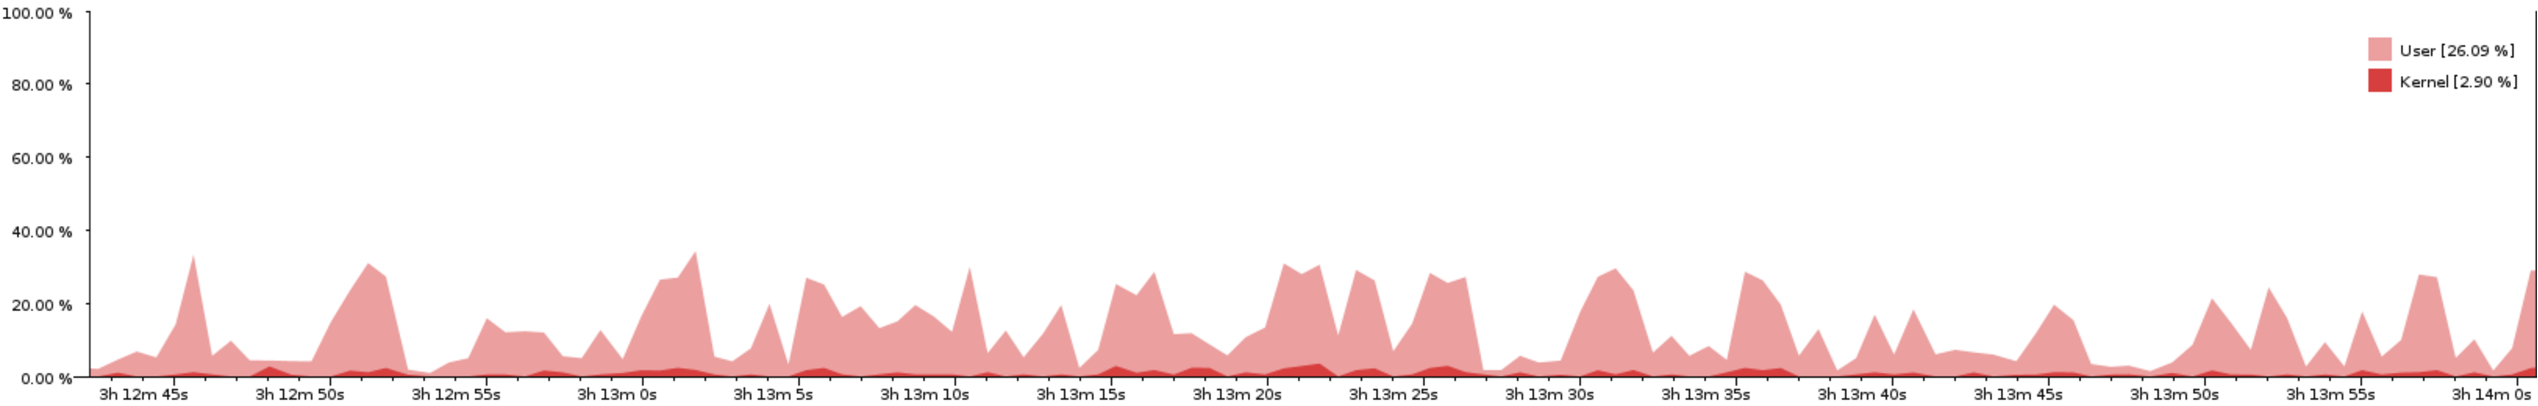
\includegraphics[scale=0.6]{monitor-cpu}
	\end{adjustbox}
	\label{fig:monitor-cpu}
\end{minipage}
~~~~~~~~~~~~~~~~~~~~
\begin{minipage}{.4\textwidth}
	\begin{adjustbox}{addcode={\begin{minipage}{\width}}{\caption{
						CPU usage on a Galaxy S3 smart-phone, about 2 minutes into the Multichain performance measurement
			}\end{minipage}},rotate=90,center}
		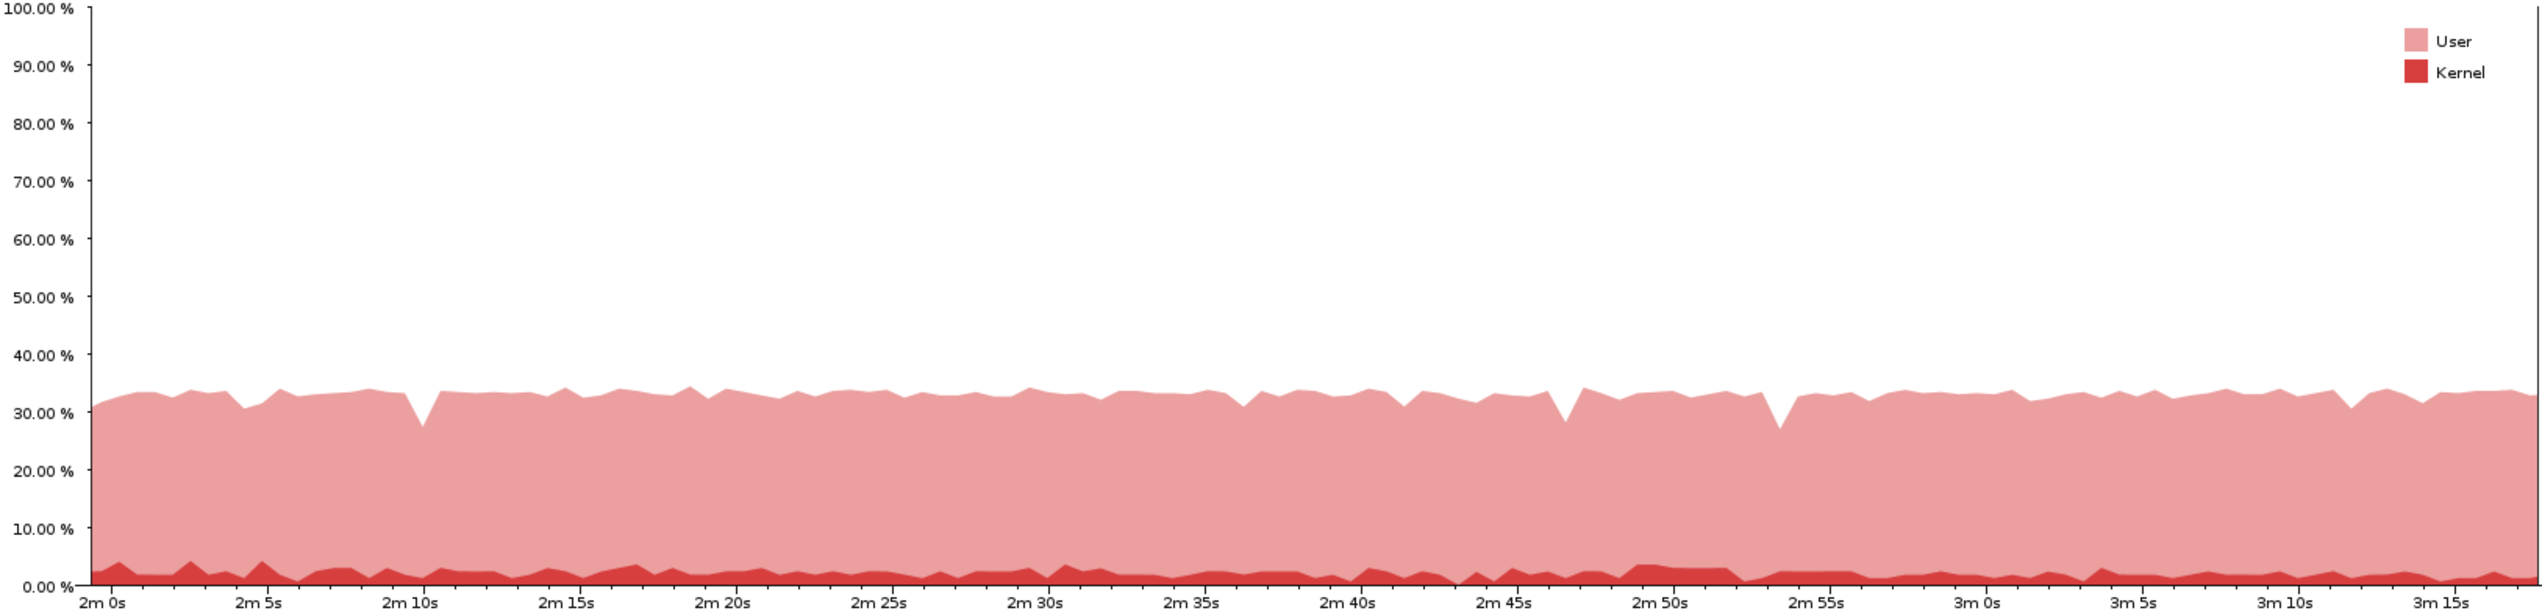
\includegraphics[scale=0.6]{monitor-cpu-experiment}
	\end{adjustbox}
	\label{fig:monitor-cpu-experiment}
\end{minipage}
\end{figure}
The results show that indeed not al 4 cores of the CPU are utilized by a large margin.
Even when performing the intensive crypto work of the Multichain experiment 2 CPU cores appear to be idling.
% Conclusions
This suggests that releasing the GIL during heavy crypto work could result in a significant performance gain.
However our results are inconclusive and warrant further research.


\section{Testing and coverage}
% Rationale
The design choice of reusing all Tribler core source code means we need to verify its correctness.
To make sure all code on Android works the same as on other supported platforms we need to test all code.
Tribler has some unit tests and integration tests that cover a large portion of the code, but not all.
% Metrics
The ratio of tested lines of code with respect to the total number of lines of code is the coverage line-rate.
% Expected / desired results
We expect to see a line-rate value close to 1, but not 1 since we know the tests do not cover everything.
% Setup
All tests were run two times on the same device with 11 weeks of development in between.
The nose module was used for running the tests together with the coverage module for gathering coverage data.
The same Nexus 6 smart-phone with Android 6.0.1 Cyanogen mod was used in both runs.
% Results
The following table shows the results of both executions.
\begin{table}
	\begin{tabular}{l | *{5}{r}} \hline
		Run & Tests & Errors & Failures & Skipped & Line-rate \\ \hline \hline
		1     & 711   & 14       & 13          & 30          & 0.7241 \\ \hline
		2     & 749   & 12       & 15          & 3            & 0.7861 \\ \hline
		3	  & 782	  & 10		 & 18		   & 4			  & 0.7871 \\ \hline
		PC   & 812   & 0         & 0            & 30          & 0.7894 \\ \hline
		PC   & 812   & 0         & 0            & 30          & 0.7901 \\ \hline
		4     & 782   & 10       & 18          & 4            & 0.7897 \\ \hline
	\end{tabular}
	\caption{Tests results and coverage line-rate at different points in time during development}
	\label{table:testing_coverage}
\end{table}
%TODO explain failures and 30 vs 4 skipped
%GUI test fail because import Qt above @skip

The number of tests has increased as well as the coverage line-rate while the number of errors and skipped tests have decreased.
A failure means an assertion was not met and an error represents an exception while running a test.
% Conclusions
Therefore seeing that the number of failures increased is not that bad since the number of errors decreased.
If the line-rate is 1 you still need the the branch-rate to be 1 as well before you can be confident the code will work as expected.
The branch-rate is the number of code paths tested with respect to the total number of code paths possible.
Unfortunately this metric is not part of the current test plan.
Nevertheless the metrics show improvement overall.

